\section{Preprocessing Data}
\label{cha:preprocessing}

In total, two datasets were used to create features for testing the different classifiers:
\textit{movies\_metadata.csv} and \textit{credits.csv}. The dataset \textit{movies\_metadata.csv} contains 45,463 rows and 23 columns excluding the id-column. The dataset \textit{credits.csv} contains 45,463 rows and 2 columns excluding the id-column.

\paragraph{Vertical scaling.}
Both dimensions for the dataset \textit{movies\_metadata.csv} were processed. As section \ref{sec:merge_create} explains, the revenue and budget played a major role for the data mining task. Therefore all datasets without information on each column had to be dropped out, which was a major part of the dataset. Also duplicates were identified using the ID and discarded. 
 
After this, the dataset shrunk to roughly 4000 rows. To retain some numbers and still use datasets which had only missing out revenue or budget two approaches were implemented: A parser for the IMDB database\footnote{
\hyperref{http://www.imdb.com/}{external_sources}{ref:IMDB}{The IMDB database: http://www.imdb.com/}} API and for the The Numbers\footnote{\hyperref{http://www.the-numbers.com/research-analysis}{external_sources}{ref:numbers}{the numbers website: http://www.the-numbers.com/research-analysis}} API was programmed and run. With these approaches it was possible to gain the real values of budget and revenue for the dataset. By mining two of the most reliable movie-datasources out in the web, it was also possible to determine rows, which used foreign currency values in their revenue or only revenue based on the local market (e.g. only in the US).

\paragraph{Horizontal scaling.}
Based on the assumptions that budget and revenue were crucial numbers, also other features have been selected for the modeling. A special focus has been placed on the following datacolumns: the release year, the genre, the production country as well as the production company, the spoken languages, the runtime and the fact whether a movie belongs to a collection or not. Due to high encoding effort for these features, further columns are not taken into account during this project. Figure \ref{img:mm_columns} gives an overview on which information was retained.

The reason why information, which could have been potentially interesting, had to be dropped, was mainly for time reasons. Preprocessing took about 70\% of the timeperiod\footnote{Mainly due to the fact that heaps of problems arose from the dataset, which can be read in chapter \ref{cha:data_selection}.} of the whole project. Thus, the team was able to focus on preprocessing of mentioned columns. Still, chapter \ref{cha:data_selection} provides a prospect, which steps were possible, if a larger time frame was dedicated to this project.

After dropping out information, eleven columns remained. Combined with the two columns from the \textit{credits.csv} dataset, thirteen columns were used as a basis to create features for finding the best performing classifiers.

In order to transform the data into a suitable representation for forecasting a movie's success, preprocessing was mandatory. For each column zero or more preprocessing steps from the following list were performed:
\\ \\
\fbox{\begin{minipage}{\textwidth}
\textit{Merging of columns, discretization (binning) of features, extracting information out of columns, one hot encoding normalizing.}
\end{minipage}}
\\ \\
The following sections explain the preprocessing in detail. Figure \ref{img:features} shows precisely, which operations were executed on each column and how the data types changed.


\paragraph{Merging and creating columns.}
\label{sec:merge_create}



When a new movie is planned, the finances are one of the most important concerns. Where the budget can be circumscribed upfront, revenue is nearly impossible to guess. As a result, the prediction of a model should consider the revenue as a key factor for it's monetary success. To only predict the revenue (using multiple bins or binary binning, like e.g. "will the revenue of a new movie be higher or lower than \$500,000?") would not have worked out due to multiple reasons: Both the revenue and budget of a movie in earlier years, like e.g. the 1950's, was
\begin{wrapfigure}{l}{0.7\textwidth}
	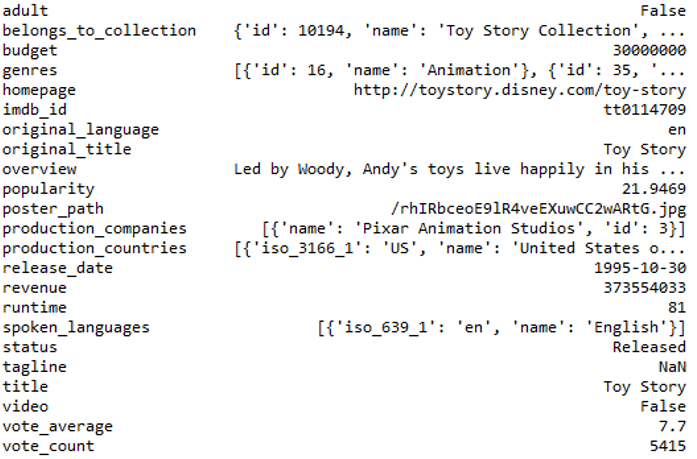
\includegraphics[width=0.7\textwidth]{images/3_metadata_columns.png}
	\caption{Remained columns of \textit{movies\_metadata.csv} are highlighted in yellow}
	\label{img:mm_columns}
\end{wrapfigure}
\FloatBarrier
 considerably less than today, so total numbers are not comparable. Additionally, inflation plays a role in comparing financial numbers of elder movies to newer ones. Furthermore, the dataset contained different currencies like dollars, euros or indian rupees without indicating which currency was provided per dataset.
 
As described in chapter \ref{sec:data_exploration}, a new column had to be introduced, namely the productivity. It is a quotient, computed by dividing revenue through budget. If the productivity is higher than one, the movie derives profit, if the productivity is less than one, the movie derives a loss. That way, above mentioned issues can be avoided. The column revenue was dropped afterwards.

Considering the release date of a movie, the assumption was made that the demand for movies is higher in quarter four of the year (time of winter and christmas). This was confirmed by checking the numbers\footnote{Check for details on revenues in video-selling: \hyperref{https://de.statista.com/statistik/daten/studie/182319/umfrage/umsatzentwicklung-im-video-kaufmarkt-quartalszahlen/}{link}{Statista revenue movies}{https://de.statista.com/statistik/daten/studie/182319/umfrage/umsatzentwicklung-im-video-kaufmarkt-quartalszahlen/}}. Hence, a new column of numeric type with quarter one to four was created. The previous column release date was converted to release year only as a numeric format.

\paragraph{Discretization.}
During this preprocessing step, the created column productivity was binned two ways: Once multi-binned into four different bins having bins between 0.0 to 0.99 (label "\textit{unproductive}"), 1.0 to 1.99 (label "\textit{smallProductivity}"), 2.0 to 4.99 (label "\textit{goodProductivity}") and 5.0 to infinity (label "\textit{highProductivity}"), and once binary-binned into two bins having 0.0 to 0.9 (label "\textit{no}") and 1.0 (label "\textit{yes}") to infinity. For each bin a new column was added, the former productivity column was dropped.

\paragraph{Extracting information.}
As stated in chapter \ref{cha:data_selection} some information, including the production companies, actors and crew members is provided as a JSON Object inside a column of the dataset. 

The first approach, taken into account contained parsing of the JSON data. However, some columns contained invalid JSON format and therefore made the processing very cumbersome.

However, after a closer analysis of the values inside the column, a new extraction concept could be developed. Given the values of the cast column, actors could be extracted by looking for the regular expressions inside the correlating values. For example actors could be identified by looking for the parameter name, and extracting the value provided by the parameter. The same procedure with slight changes has been applied to the extraction of the production companies, the directors and the countries of production.

After evaluation of the extracted parameters, inconsistent values for the production companies have been discovered. These inconsistent values contain for example: "Twenty Century Fox", "Twenty Century-Fox" and "Twenty Century Fox Production". Without any further preprocessing each of the values would be one hot encoded separately. Therefore a second step of preprocessing has been performed to remove different ways of writing the same company, and therefore providing similar values for one hot encoding.
 
\paragraph{Normalizing, thresholding and one hot encoding.}
Not only the in the previous step extracted information on genre, production country, production company director and actor was one hot encoded using the pandas get\_dummies()\footnote{The \hyperref{https://pandas.pydata.org/pandas-docs/stable/generated/pandas.get_dummies.html}{documentation}{pd.getDumies}{Documentation on pandas get\_dummies() function can be found online}} function, but also the original language. After one-hot-encoding, the dataset consisted of about 49000 columns\footnote{The high number is due to the high number of different actors, directors, production companies and production countries.}.

In order to reduce the amount of columns and to filter out unnecessary data a threshold had been applied. For example actors, directors and companies, which are not frequently participating in the movie-production-scene have been eliminated using a filter. Thus it can be assured that only actors et. al are taken into account which participated in a reasonable amount of movies, and therefore have an impact on the classifier.

In order to create equal meaning among the different numeric values in the data set some of the columns, including runtime, budget and year, are normalized using MinMax scaling.

\begin{figure}[htbp]
	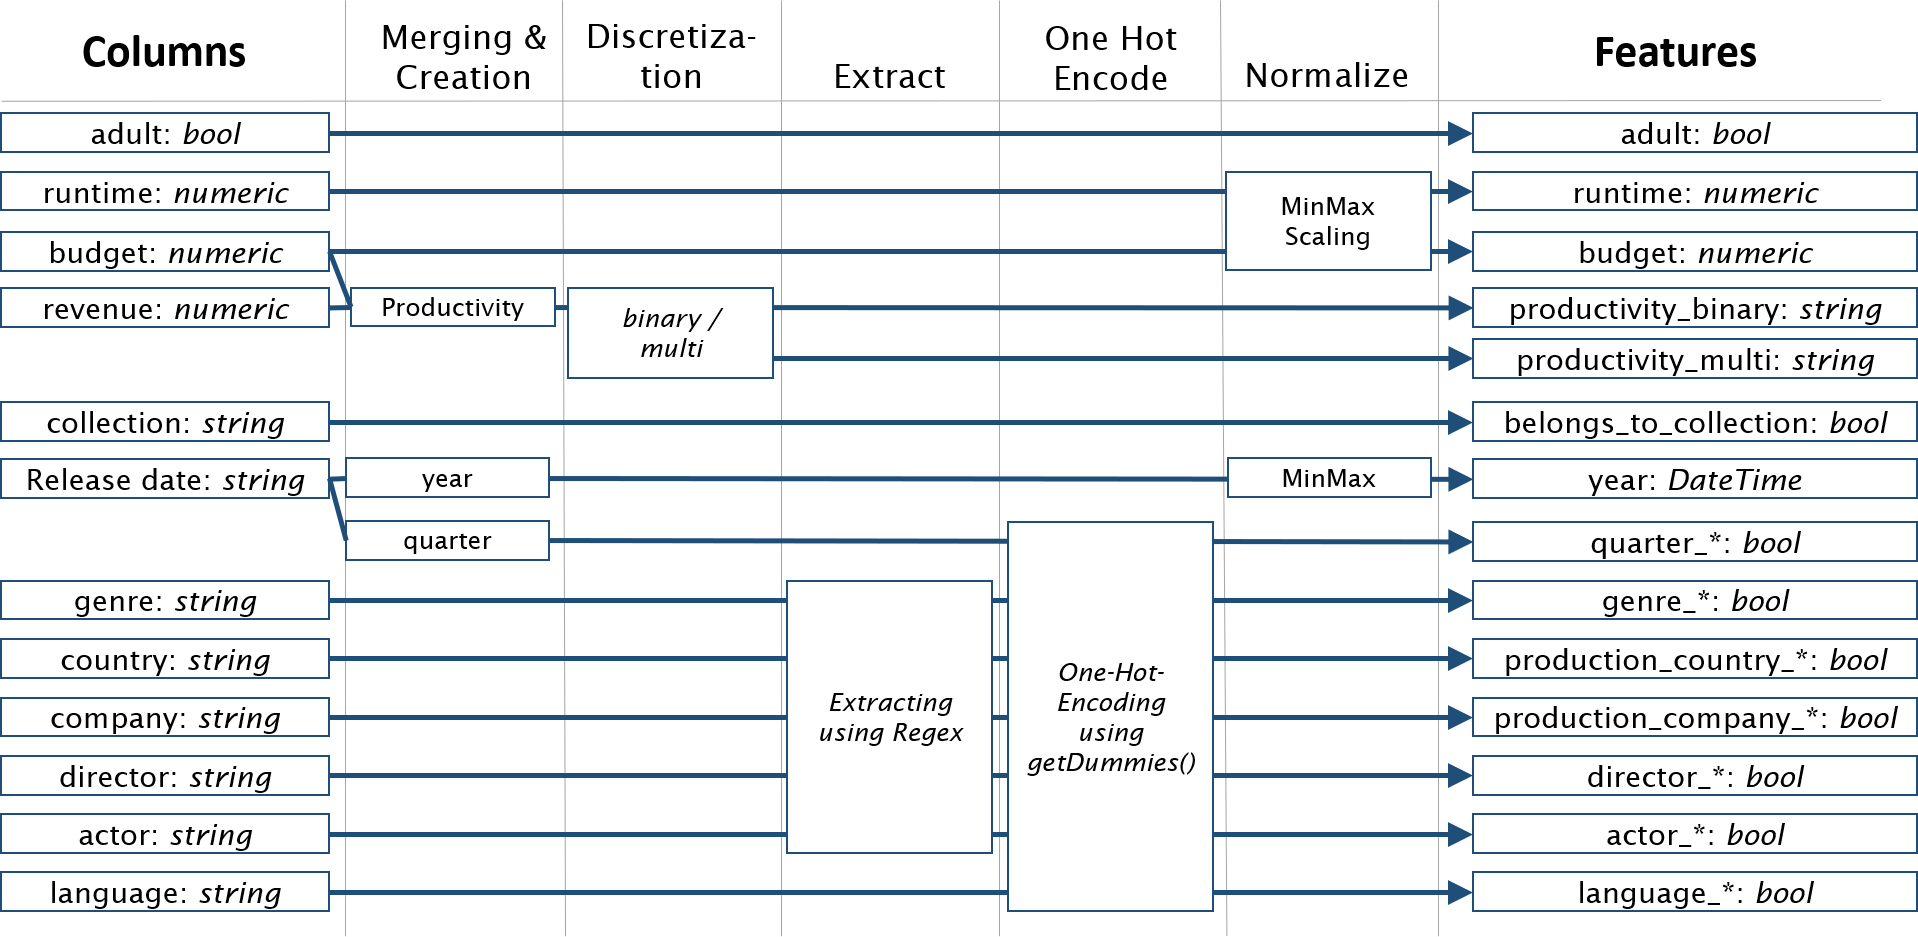
\includegraphics[width=\textwidth]{images/3_features.png}
	\caption{Features created during preprocessing}
	\label{img:features}
\end{figure}
\FloatBarrier

%\begin{itemize}
%	\item Transform data into a representation that is suitable for the chosen data mining methods
%	\begin{itemize}
%		\item number of dimensions
%		\item scales of attributes (nominal, ordinal, numeric)
%		\item amount of data (determines hardware requirements)
%	\end{itemize}
%	\item Methods
%	\begin{itemize}
%		\item Aggregation, sampling
%		\item Dimensionality reduction / feature subset selection
%		\item Attribute transformation / text to term vector
%		\item Discretization and binarization
%	\end{itemize}
%	\item Good data preparation is key to producing valid and reliable models
%	\item Data preparation estimated to take 70-80\% of the time and effort of a data mining project!
%\end{itemize}

%\section{A list of problems we encountered}
%\begin{enumerate}
%	\item \textbf{list further problems we had and solved!}
%	\item Prod. Comp.: Same prod. company named differently -> using Regex to solve (Steffen)
%	\item dataset: 5 datasets have duplicates
%\end{enumerate}
